% !TeX program = xelatex
\documentclass[UTF8,11pt,a4paper,linespread=1]{ctexart}
\usepackage[margin=26mm]{geometry}
\usepackage{amsmath,amssymb,bm}
\usepackage{setspace}
\setstretch{1.35}
\usepackage{pgfplots,booktabs}
\pgfplotsset{compat=1.18}
\usepackage[unicode,colorlinks=true,linkcolor=teal,urlcolor=teal]{hyperref}

\begin{document}
\section{从一个积分连接到图和表}\label{sec:demo}
\begin{equation}\label{eq:area}
  \int_0^1 x^2\,\mathrm{d}x=\frac13.
\end{equation}

\begin{figure}[htbp]
  \centering
  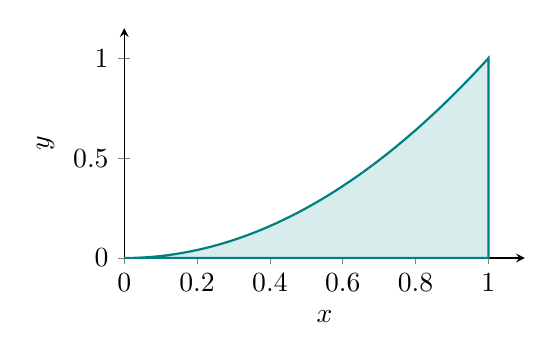
\begin{tikzpicture}
  \begin{axis}[width=.55\linewidth,height=4.5cm,axis lines=left,
    xmin=0,xmax=1.1,ymin=0,ymax=1.15,xlabel={$x$},ylabel={$y$}]
    \addplot[teal,thick,fill=teal!15,domain=0:1,samples=51]{x^2}\closedcycle;
  \end{axis}
  \end{tikzpicture}
  \caption{区间 $[0,1]$ 上的平方函数及其下方面积}\label{fig:demo}
\end{figure}

\begin{table}[htbp]
  \centering
  \caption{积分结果的记录}\label{tab:result}
  \begin{tabular}{lc}
    \toprule
    项目 & 结果 \\
    \midrule
    定积分 & $1/3$ \\
    \bottomrule
  \end{tabular}
\end{table}

式~\eqref{eq:area} 给出精确积分值；
图~\ref{fig:demo} 和表~\ref{tab:result} 分别展示插图与结果表。
也可以点击\hyperref[sec:demo]{这段文字返回本节开头}。

\end{document}
